\section{Étape 2: Caractérisation des plateformes}\label{sec:methodo_step2}
%%%%%%%%%%%%%%%%%%%%%%%%%%%%%%%%%%%%%%%%%%%%%%%%%%%%%%%%%%%%%%%%%%%

Lors de la première étape, les caractéristiques des plateformes ont été calculées pour sélectionner celles avec le meilleur potentiel. Pour l'étape deux, il est nécessaire d'avoir accès aux différentes architectures pour réaliser une caractérisation fine de leur comportement et de leurs performances.

\subsection{Introduction}
%%%%%%%%%%%%%%%%%

    \subsubsection{Performance de référence}
    %%%%%%%%%%%%%%%%%%%%%%%%%
        
        Pour pouvoir estimer la bonne ou mauvaise performance d'un code sur une plateforme, il est nécessaire d'avoir une performance de référence avec laquelle la comparer. Grâce à cette référence, il est ensuite possible d'estimer les gains de performance dont pourrait profiter une application son portage sur une nouvelle architecture ou son optimisation. Un modèle largement utilisé dans le domaine de l'analyse de performance est celui du Roofline, présenté dans la \autoref{sec:roofline}. Pour sa construction, il faut disposer de deux caractéristiques de l'architecture: le débit mémoire ($GB/s$) et le débit de calculs ($FLOP/s$). Pour les obtenir, deux méthodes sont possibles (voir \autoref{sec:methodo_step2}). La première est de la calculer à partir des données techniques de l'architecture et la deuxième est de la mesurer.
        
        \paragraph{Objectif.} L'objectif de cette deuxième étape est donc d'obtenir ces valeurs de références pour pouvoir projeter et apprécier les performances d'une application. 

        \begin{figure}[h!]
        \center
        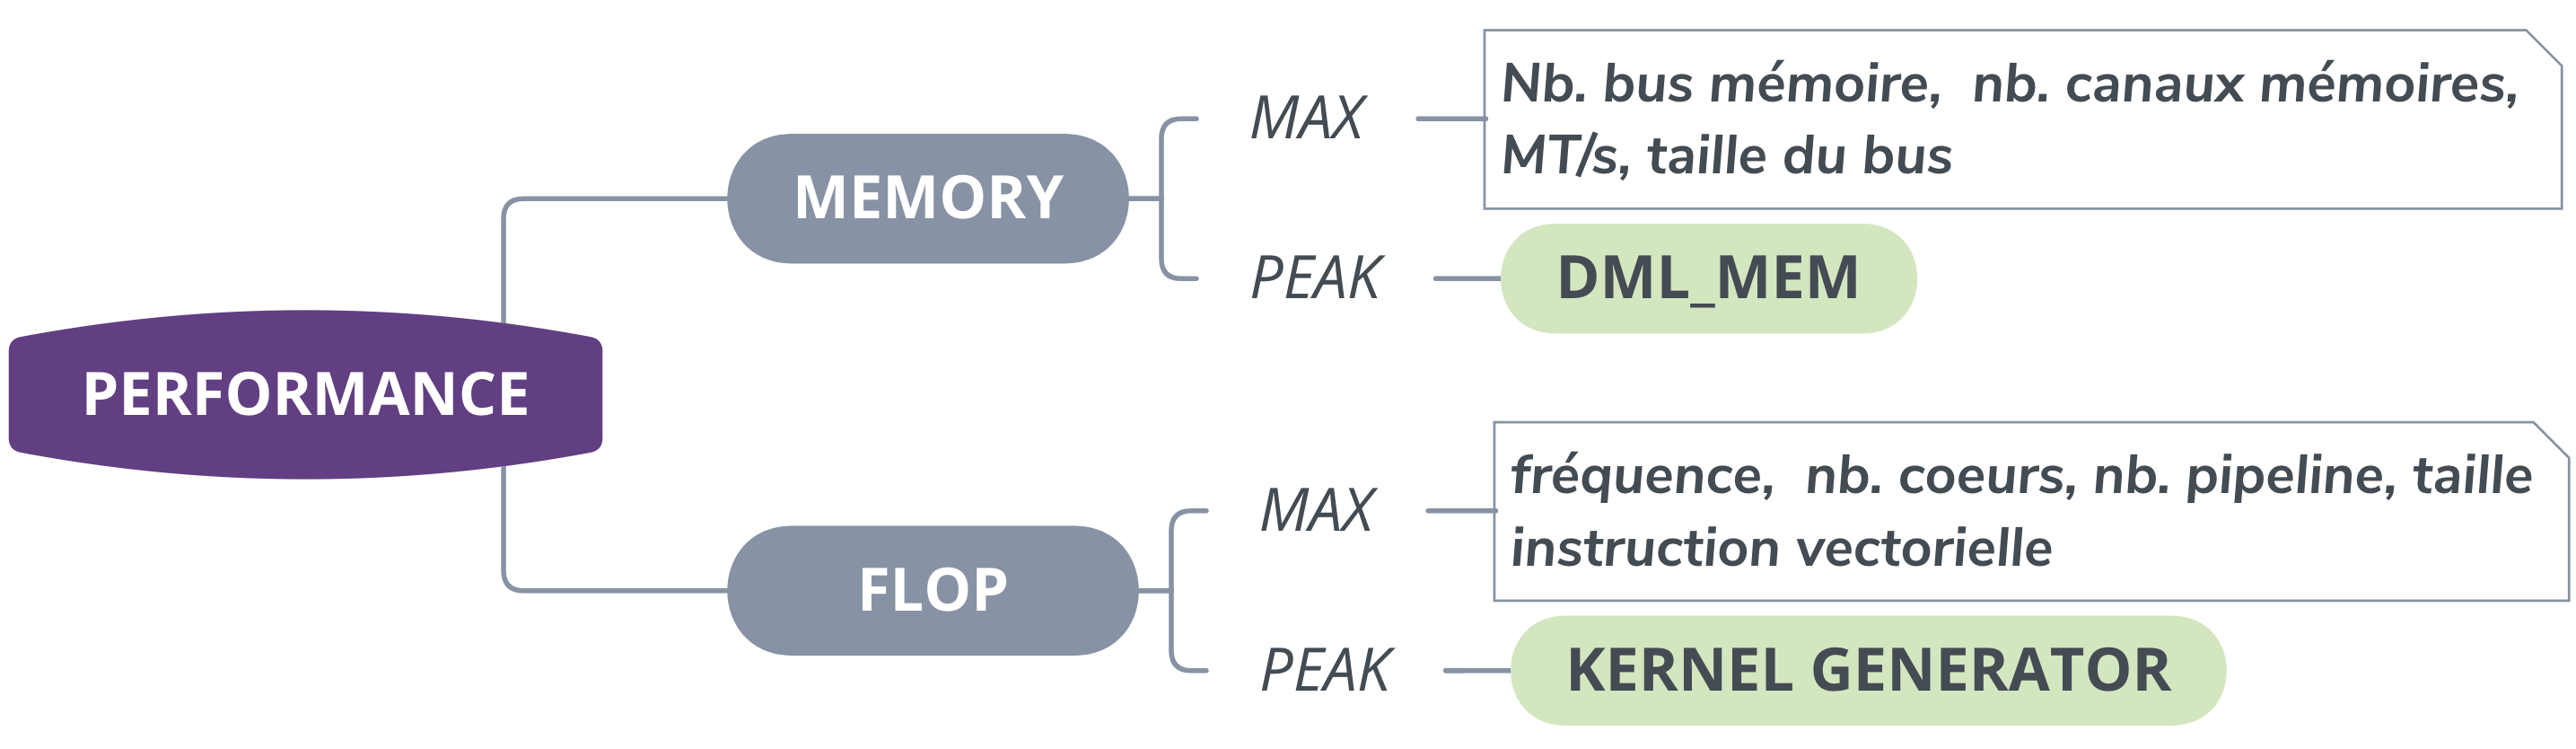
\includegraphics[width=14cm]{images/methodo_step2.png}
        \caption{\label{pic:methodo_step2}Caractériser les plateformes en calculant la performance théorique et en mesurant la performance crête.}
        \end{figure}


    \subsubsection{Performance maximale théorique}
    %%%%%%%%%%%%%%%%%%%%%%%%%%%
        
        L'implémentation \textit{naïve}\cite{Williams2008a} du modèle du Roofline utilise les performances théoriques de la microarchitecture. Celle du système mémoire est notée ($\text{MEMORY}_{peak}$) et celle du processeur ($\text{FLOP}_{peak}$). Malheureusement, à cause de la complexité des architectures, il est très rare qu'une application atteigne une performance égale à la performance théorique. Même des applications spécialisées telles que \verb=STREAM= et \verb=LINPACK= n'y parviennent pas. Il est donc très rare de voir des applications industrielles atteindre la performance maximale théorique notée $\text{PERF}_{peak}$.
    
        
    \subsubsection{Performance maximale mesurée}
    %%%%%%%%%%%%%%%%%%%%%%%%%%%
    
        Pour caractériser une nouvelle architecture, il est donc plus précis de mesurer ses performances. Une application industrielle peut être difficile à porter sur une nouvelle architecture. Il est donc peu recommandé de réaliser ce portage dans le simple but de caractériser cette dernière. Il est préférable d'utiliser des benchmarks, plus courts et plus facilement portables. Après le portage de l'application sur la plateforme choisie, il sera possible de comparer la performance mesurée de l'application, notée $\text{PERF}_{max}$\protect\footnotemark, avec la performance maximale atteignable ($\text{PERF}_{peak}$\textsuperscript{\ref{note1}}).

    
        Pour obtenir les deux caractéristiques qui nous intéressent ici (notées $\text{MEMORY}_{max}$ et $\text{FLOPS}_{max}$), il est courant d'utiliser des benchmarks de références. Par exemple pour mesurer la bande passante mémoire maximale atteignable on peut utiliser le benchmark \textit{Stream} \cite{McCalpin1995}, les latences des différents niveaux de caches \textit{lmbench} \cite{Staelin2002}. Pour mesurer le nombre maximum d'opérations sur un nombre flottant exécutable par seconde, on peut utiliser le benchmark LINPACK.
        
        L'avantage de cette approche est sa facilité. Il suffit de compiler le benchmark voulu et de l'exécuter pour obtenir les résultats. L'inconvénient est que la mesure est dépendante de la qualité du code et du compilateur. Il peut arriver qu'en voulant mesurer spécifiquement un composant, les performances soient dégradées par une autre partie de la microarchitecture. Par exemple, si l'on cherche à mesurer la bande passante maximale atteignable par un seul coeur avec un code simple lisant un tableau de données. Sur un processeur récent tel qu'un Xeon Skylake, on s'attendrait à obtenir une valeur proche du maximum théorique de 128 GB/s, calculé dans lors de l'étape précédente. Cependant, à cause de la Loi de Little \cite{little2008little} et de la taille de la queue de chargement (\textit{outstanding load queue}), il faut plus de dix coeurs actifs pour saturer la bande passante \cite{JohnMcCalpin2010}. Il faut donc une certaine expérience des outils et des microarchitectures pour apprécier les résultats mesurés. Il peut ainsi être nécessaire d'avoir plusieurs codes de benchmark à exécuter pour valider de différente façon le comportement de la microarchitecture.
        
        \footnotetext{\label{note1}Le classement du Top500 utilise les notations $\text{R}_{max}$ et $\text{R}_{peak}$ pour   désigner la performance maximale atteignable et la performance maximale théorique d'un supercalculateur.}


  
%%%%%%%%%%%%%%%%%
\subsection{Application au processeur Intel Xeon 6148}
%%%%%%%%%%%%%%%%%
    
    Nous présentons ici comment les outils développés durant la thèse permettent de caractériser la microarchitecture du processeur Intel Xeon Skylake 6148. Nous mesurons le débit mémoire maximale du bus mémoire ($\text{MEMORY}_{max}$) à l'aide de \verb=DML_MEM= (voir \autoref{sec:yamb}) et la puissance de calcul du processeur ($\text{FLOPS}_{max}$) grâce au \verb=Kernel Generator= (voir \autoref{sec:kg}).


    \subsubsection{Débit mémoire maximal}
    %%%%%%%%%%%%%%%%%%%%%%%%%%%%%%%%%%%%
        
        Pour caractériser le système mémoire du processeur, nous paramétrons l'outil \verb=DML_MEM= pour réaliser des accès mémoire avec des sauts en mémoire de la taille d'une ligne de cache.
        Pour nous assurer de la capacité du processeur à générer suffisamment de transactions mémoires pour saturer le bus (voir Loi de Little \autoref{sec:loidelittle}), nous exécutons le benchmark sur les 20 coeurs disponibles. La commande résultante pour cette expérimentation est la suivante:
\begin{lstlisting}
mpirun -np 20 numactl dml_mem  --steplog 0 --unroll 8 
                               --type read --stride 64 --matrixsize 5000
\end{lstlisting}
        Lors de l'étape 1, nous avions calculé une performance crête théorique $\text{MEMORY}_{peak}$ de 128 GB/s. A l'aide de \verb=DML_MEM=, nous obtenons une bande passante mémoire $\text{MEMORY}_{max}$ de 105 GB/s.
        
    
    
    \subsubsection{Performance de calculs}
    %%%%%%%%%%%%%%%%%%%%%%%%%%%%%%%%%%%% 
    
        Pour mesurer la performance maximale atteignable ($\text{FLOPS}_{max}$) par le processeur, nous utilisons le générateur de benchmark \textit{Kernel\_Generator}. Nous avons paramétré le générateur pour évaluer le nombre maximum d'opérations \gls{FMA} AVX-512 réalisable sur un nombre flottant à double précision. Pour cela nous avons utilisé la commande présentée ci-dessous. Nous générons un kernel de 14 instructions FMA pour réduire le coût de gestion de la boucle (incrémentation et comparaison) et masquer la latence des instructions.

\begin{lstlisting}
./kg -W 512 -O ffffffffffffff -P double -S 100 -L 120000000
\end{lstlisting}
        
        Le benchmark généré ne possède pas de version multicoeur, nous lançons donc indépendamment 20 exécutions du binaire que l'on accroche à un coeur différent grâce à un paramètre du benchmark. Pour cette expérience nous avons commencé par désactiver le turbo du processeur, et limité sa fréquence à 1.6GHz. La performance mesurée est de 998.57 GFLOP/s. Ensuite nous avons activé le turbo, et laissé le processeur choisir lui même sa fréquence. L'\autoref{code:kg_512_output} montre les résultats donnés par le benchmark pour l'exécution sur un des 20 coeurs. Le benchmark mesure sa fréquence effective et trouve bien la valeur de 2.2 GHz renseignée par Intel dans sa documentation. La performance maximale d'un coeur mesurée  est de 69.2 GFLOP/s, approchant le maximum théorique de 70 GFlop/s calculé dans l'étape précédente.
        
        
\begin{lstlisting}[caption=Résultat de l'exécution du benchmark sur un coeur avec le turbo activé, label={code:kg_512_output},
  basicstyle=\footnotesize, frame=tb,
  xleftmargin=.005\textwidth, xrightmargin=.005\textwidth]
------------------  INSTRUCTIONS SUMMARY ------------------------------
_label_|   NB INSTRUCTIONS      Time    FREQUENCY    inst/sec       IPC
_value_|      168000000000      38.8          2.2     4.33e+9      2.01
----------------------  FLOP SUMMARY  ---------------------------------
 PRECISION     FLOP/cycle         FLOP/second
    Single              0                   0
    Double           32.0            6.92e+10
-----------------------------------------------------------------------
\end{lstlisting}
        
        Le benchmark du \verb=Kernel Generator=, ne possède pas de version multicoeurs et ne présente que les résultats de la performance d'un coeur. Pour nous assurer que l'exécution du code sur les différents coeurs, nous avons utilisé un outil développé chez HPE appelé \textit{mygflops.sh}. Il permet de compter les instructions flottantes simples et doubles précisions exécutées sur un processeur. Le résultat est présenté dans l'\autoref{code:mygflops_512_output}. La performance maximale mesurée du processeur $\text{FLOPS}_{max}$ est de 1372.78 GFlop/s, proche du maximum théorique $\text{FLOPS}_{peak}$ de 1408 GFLOP/s, calculée lors de l'étape 1.
        
\begin{lstlisting}[caption=Résultat de l'outil \textit{myflops.sh} utilisé pour compter les instructions flottante exécutées sur un processeur., label={code:mygflops_512_output},
  basicstyle=\footnotesize, frame=tb,
  xleftmargin=.005\textwidth, xrightmargin=.005\textwidth]
Single-precision SSE/AVX :       0.00 GFlop/s  --   0.0% of Flops
Double-precision SSE/AVX :     (*\bfseries 1372.78 GFlop/s*)  -- 100.0% of Flops
   0.0% scalar  64-bit SSE/AVX instructions (  0.0% of fp instructions)
   0.0% packed 128-bit SSE/AVX instructions (  0.0% of fp instructions)
   0.0% packed 256-bit AVX instructions     (  0.0% of fp instructions)
 100.0% packed 512-bit AVX instructions     (100.0% of fp instructions)
\end{lstlisting}